\begin{frame}
    \begin{exampleblock}{Exercise VI}
        \begin{enumerate}
            \item Create an Arduino\textregistered{} \acs{iot} Cloud project.
            \item Setup and connect your board with the Arduino \acs{iot} Cloud.
            \item Read and update \acs{imu} sensor values.
            \item Control the on-board \acs{rgb} \acs{led}.
        \end{enumerate}
        \par Hint:
        \begin{itemize}
            \item \href{https://docs.arduino.cc/tutorials/nano-rp2040-connect/rp2040-iot-cloud}{Setting up Nano RP2040 Connect with Arduino\textregistered{} IoT Cloud}
        \end{itemize}
    \end{exampleblock}
\end{frame}

\begin{frame}{Solution: Exercise VI}
    \begin{exampleblock}{}
        \begin{enumerate}
            \item Open the \href{https://create.arduino.cc/iot/}{Arduino\textregistered{} \acs{iot} Cloud}.
            \item Add the board as a device.
            \item Create a thing.
                  \begin{enumerate}
                      \item Select a device
                      \item Select the network
                      \item Add variables to synchronize
                  \end{enumerate}
            \item Edit and upload the sketch
            \item Create a dashboard
        \end{enumerate}
        \par Hint:
        \begin{itemize}
            \item \href{https://docs.arduino.cc/tutorials/nano-rp2040-connect/rp2040-upgrading-nina-firmware}{Upgrading Nano RP2040 Connect NINA Firmware}
        \end{itemize}
    \end{exampleblock}
\end{frame}

\begin{frame}{Solution: Exercise VI}
    \begin{figure}
        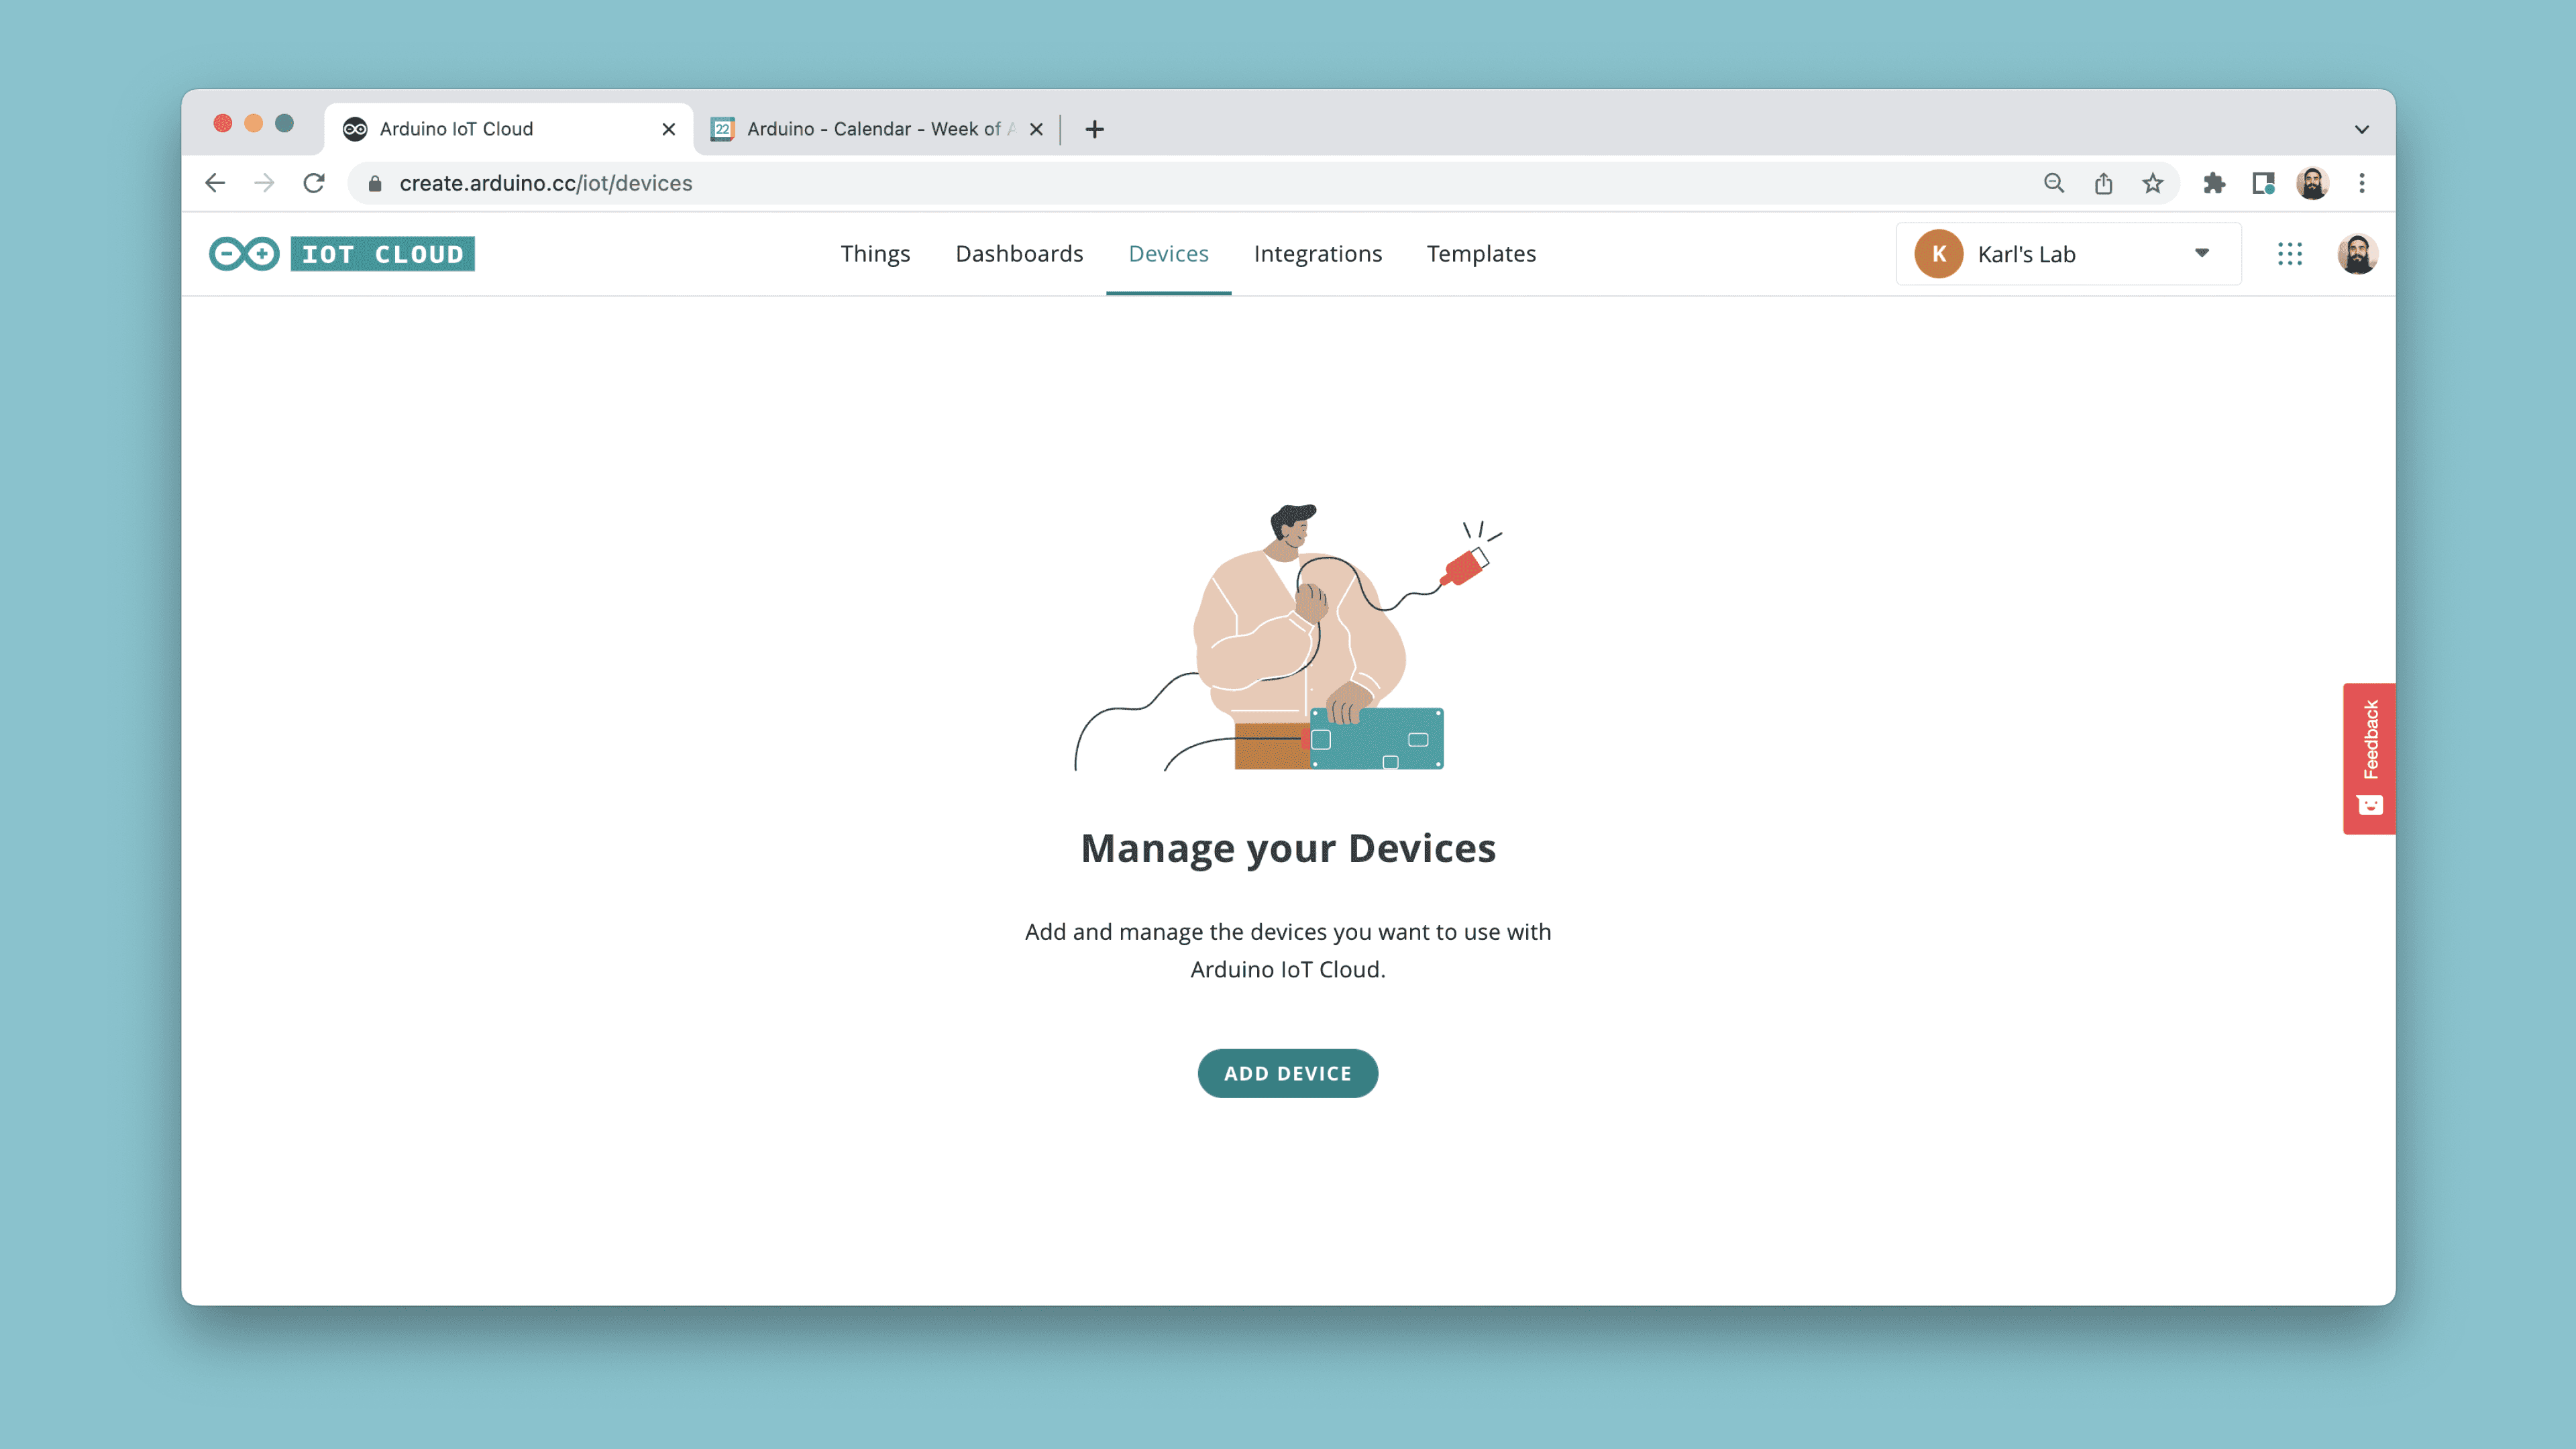
\includegraphics[width=0.95\textwidth]{images/microcontroller/iot-cloud/devices.png}
        \caption{Arduino\textregistered{} \acs{iot} Cloud: Device.}
    \end{figure}
\end{frame}

\begin{frame}{Solution: Exercise VI}
    \begin{figure}
        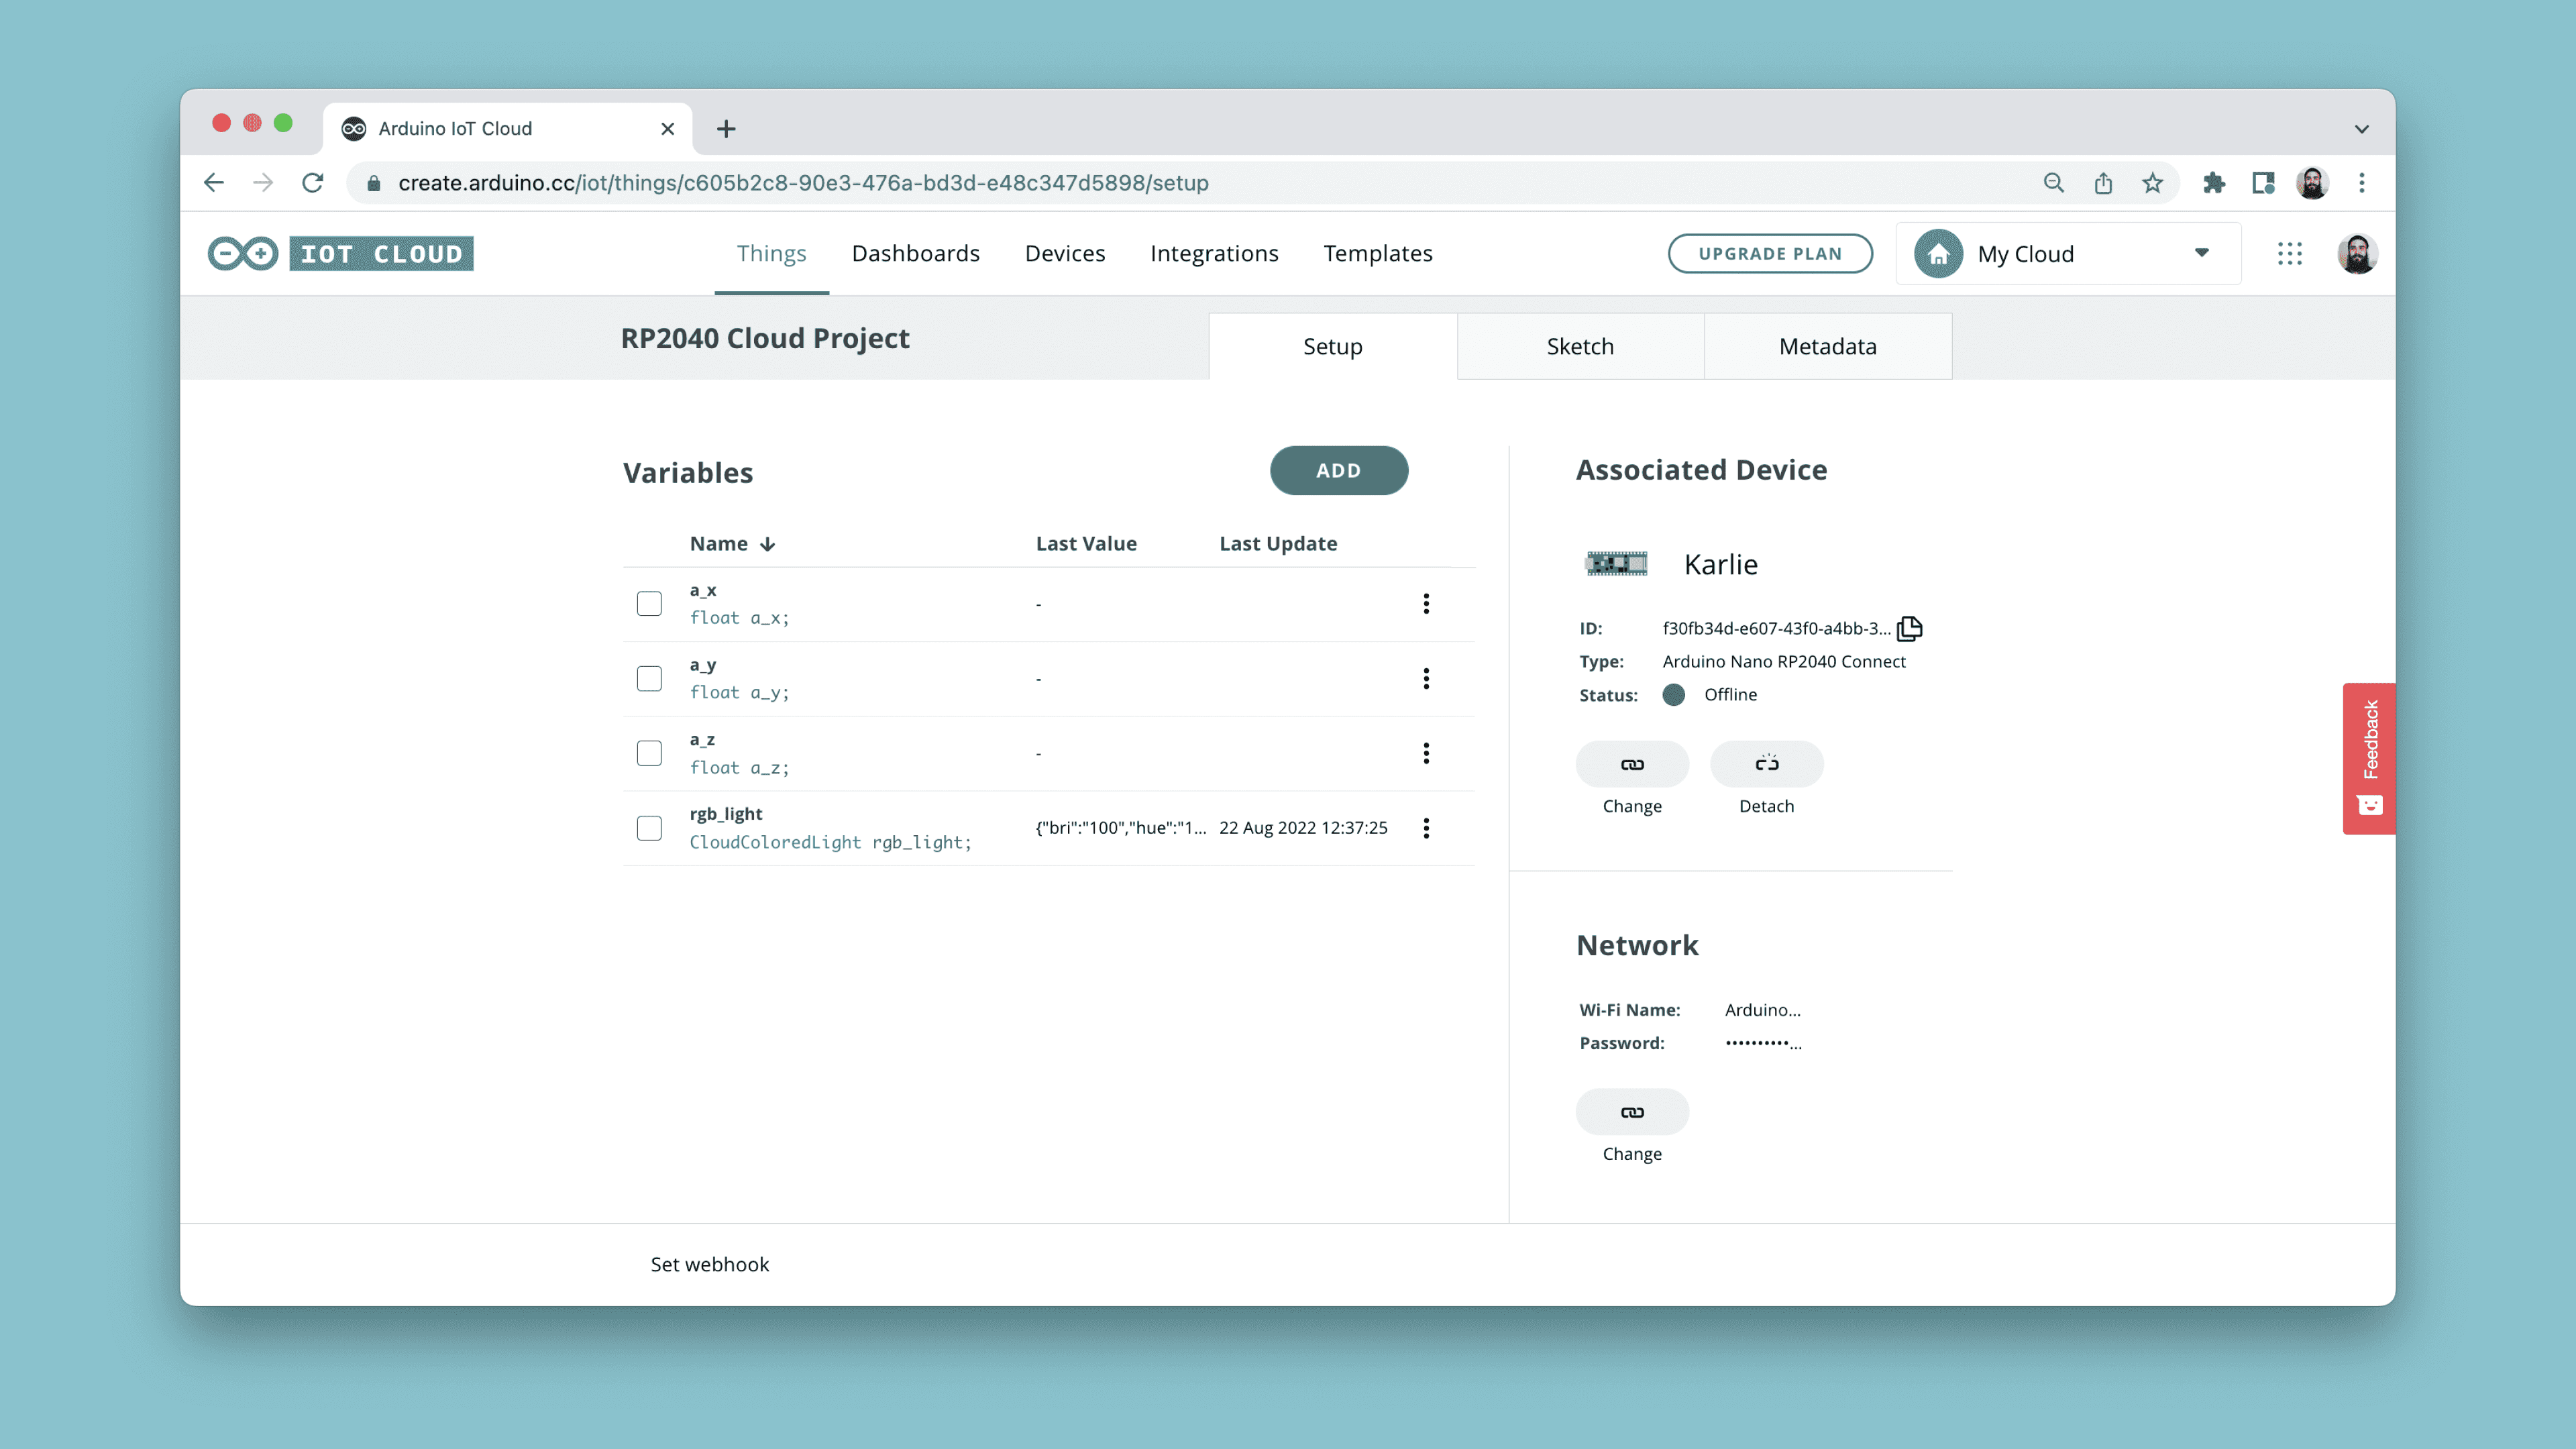
\includegraphics[width=0.95\textwidth]{images/microcontroller/iot-cloud/things.png}
        \caption{Arduino\textregistered{} \acs{iot} Cloud: Thing.}
    \end{figure}
\end{frame}

\begin{frame}{Solution: Exercise VI}
    \begin{figure}
        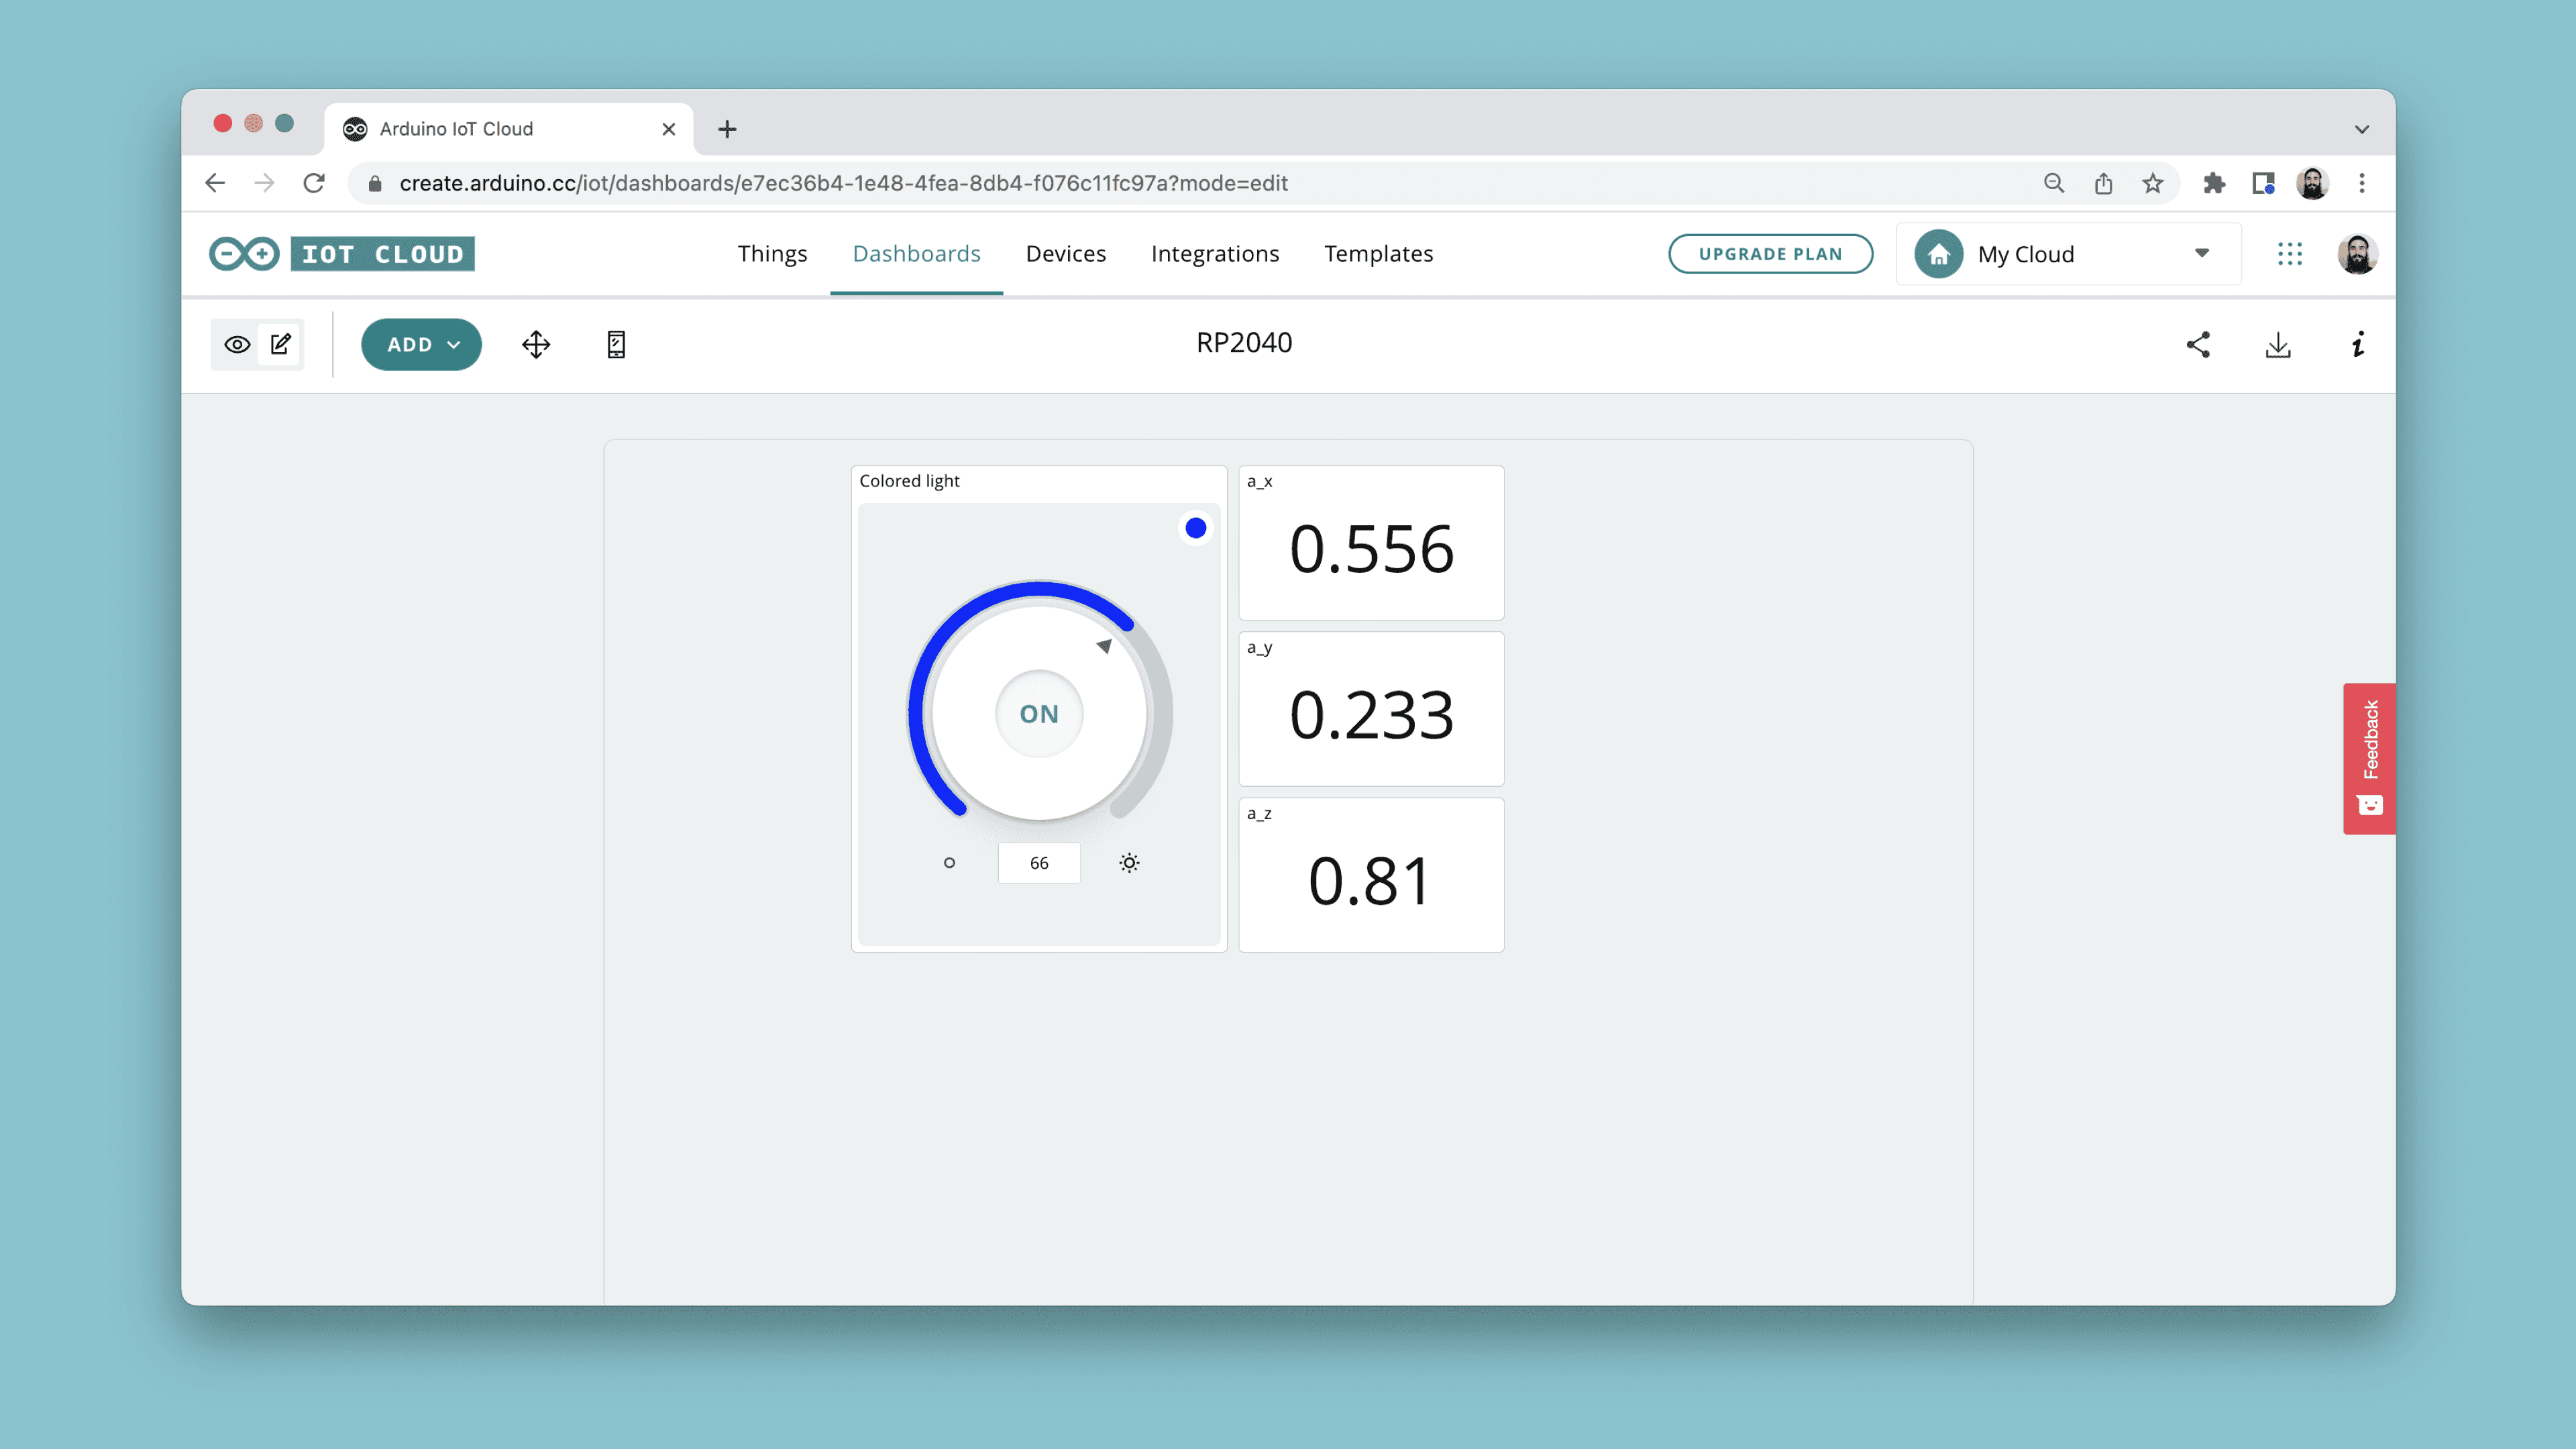
\includegraphics[width=0.95\textwidth]{images/microcontroller/iot-cloud/dashboard.png}
        \caption{Arduino\textregistered{} \acs{iot} Cloud: Dashboard.}
    \end{figure}
\end{frame}

\begin{frame}{Solution: Exercise VI}
    \begin{listing}[H]
        \inputsource[fontsize=\fontsize{7}{7}, breaklines, lastline=33]{c}{arduino/iot-cloud-rgb-imu.c}
        \caption{Solution for Exercise VI (\mintinline{c}{setup()}).}
        \label{lst:arduino:exercise:6:solution:setup}
    \end{listing}
\end{frame}

\begin{frame}{Solution: Exercise VI}
    \begin{listing}[H]
        \inputsource[fontsize=\fontsize{7}{7}, breaklines, firstline=35]{c}{arduino/iot-cloud-rgb-imu.c}
        \caption{Solution for Exercise VI (\mintinline{c}{loop()}).}
        \label{lst:arduino:exercise:6:solution:loop}
    \end{listing}
\end{frame}

\begin{frame}{Solution: Exercise VI}
    \begin{listing}[H]
        \inputsource[fontsize=\fontsize{8}{8}, breaklines]{c}{arduino/iot-cloud-properties.c}
        \caption{Solution for Exercise VI (\texttt{thingProperties.h}).}
        \label{lst:arduino:exercise:6:solution:thing_properties}
    \end{listing}
\end{frame}